%pose estimation
\chapter{Activity Recognition}
\label{activityRecognition}

\section{Introduction}

In this section we turn to the problem of recognising and clustering various activities across a range of conditions. We describe an activity as a short sequence of motion, typically undertaken by a person, and captured by either video cameras or a motion capture system. Activity recognition is an important field of study, due to the growing demand for systems that can reliably infer behaviour in a range of settings. There are a wide variety of applications for activity recognition systems. For example in home care scenarios, where robots may be employed to care for the elderly or for the disabled. In home care, the primary consideration is monitoring the status of the patient, to infer, for example, whether they are injured or safe, whether they are cooking or excersing, and most importantly, whether their behaviour appears to be normal.

In a similar fashion to previous sections, activity recognition may be used for gaming applications, for example to recognise particular movements that correspond to game commands or to infer the state of the user from their motion. 

We may also wish to employ activity recognition systems at construction sites. In large workplaces there will be a large number of hazards, for example machinery operating, uncovered holes dug in the ground, and materials swinging through the air as it is transported. This clearly presents significant danger to people as they move about construction sites. It is desirable, therefore, to employ systems that are capable of inferring the trajectory and likely behaviour of people and machinery as they move around. Systems that can identify when someone is walking and discern some information from their gait may also be useful in biometric applications, for instance in security systems, or for use with autonomous vehicles to identify the behaviour of pedestrians.



\section{Activity Recognition}


\subsection{Synthetic Function Matching with HSIC}

The principle contribution of this section is to demonstrate that our HSIC based measure provides a robust measure of the similarity between two arbitrary time-series signals. We demonstrate this capability with a series of examples on synthetic data, with a particular focus on the three main components of a signal, the frequency, the amplitude and the phase. Specifically, we show that our normalised measure is robust to changes in the amplitude, which the elementary HSIC is not. As a proof of concept we demonstrate that our measure could be used to re-construct a signal from data, in cases where Fourier based methods are not suitable. 

We are interested in matching time-series signals of various human activities. We are using motion capture data from the Carnegie Mellon dataset, which includes a wide range of activities, for example: walking, running, dancing, climbing over obstacles, swimming motions, getting up off the ground and sweeping motions. The motion capture data contains the angle of each joint over time, as well as the spatial coordinates of a root node. In order to situate our synthetic examples, we first show some examples of real motion capture data. The first two examples, shown in Fig. \ref{getting_up} are of a subject getting up off the ground from a lying position. The second two examples, shown in Fig. \ref{walks} are of a subject walking in a normal fashion. The goal of our algorithm is to measure the similarity between any two motion inputs. We show that our HSIC measure is capable of discriminating between various motions, however we typically require that the motion is first projected into a lower dimensional space. Before we demonstrate our results we will first give an overview of principle component analysis.

\begin{figure}
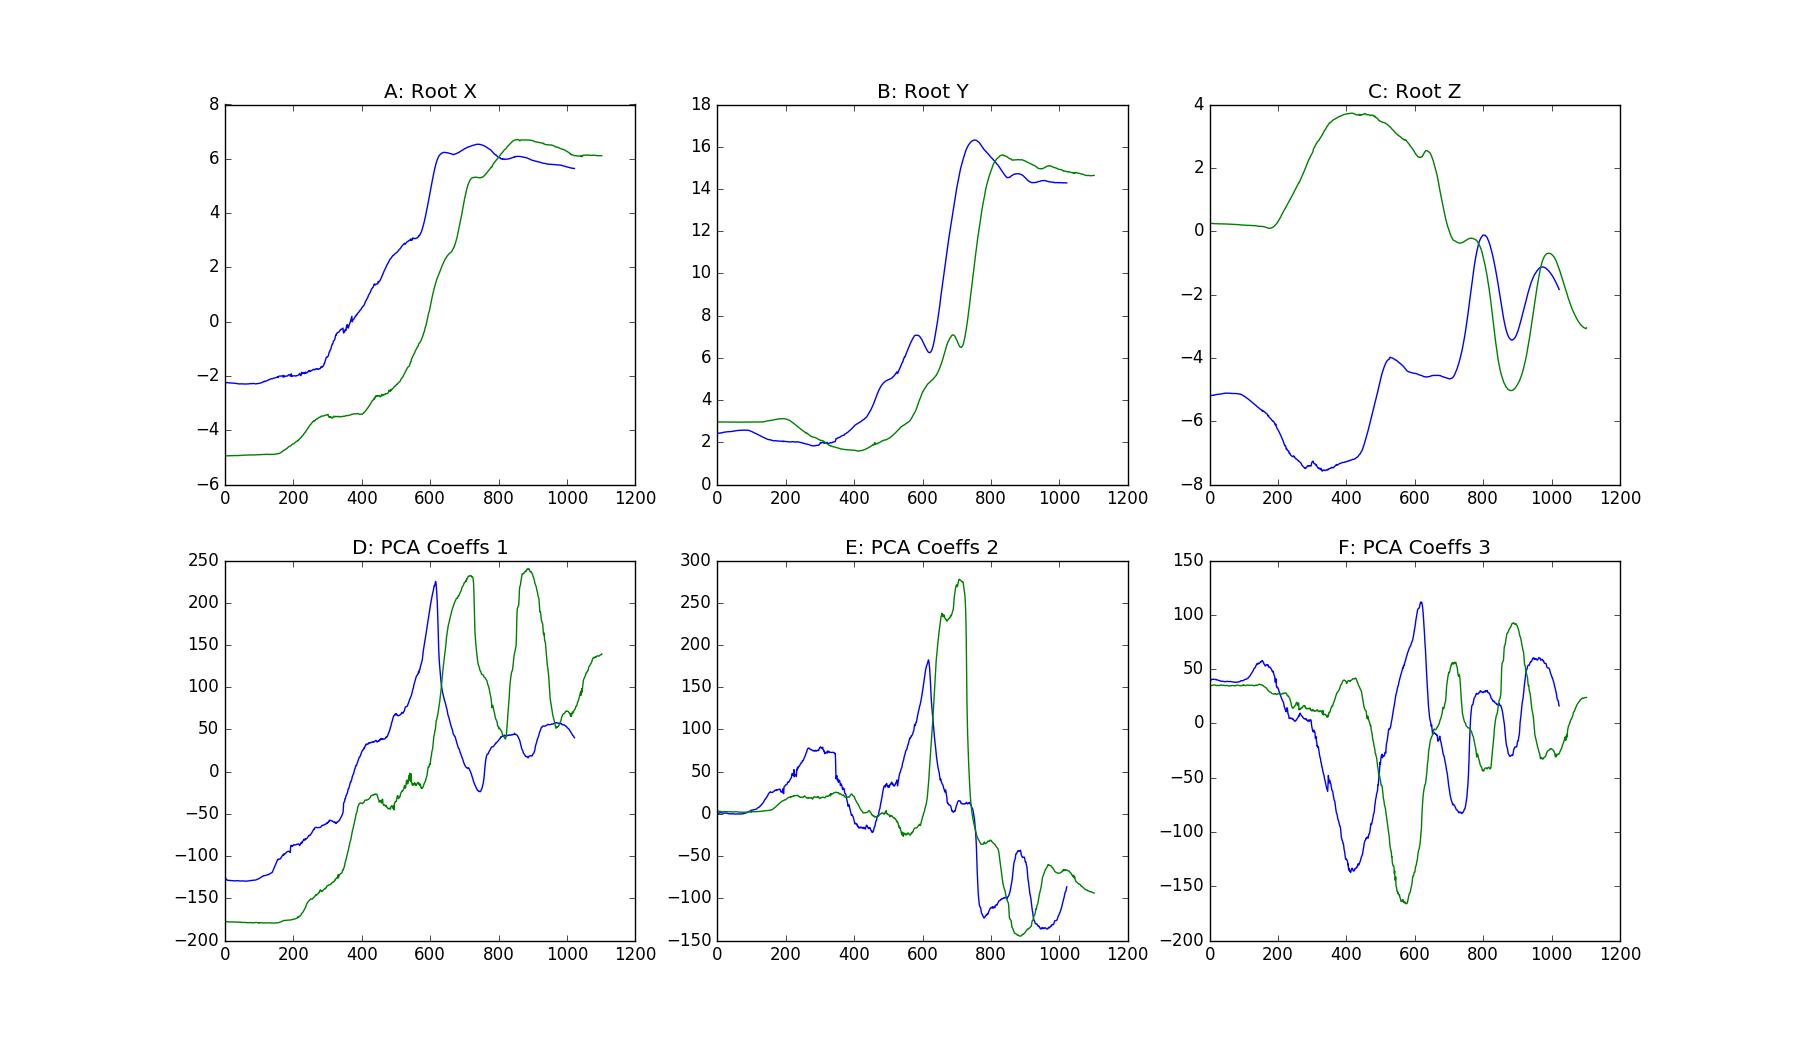
\includegraphics[width=\textwidth]{/home/cshome/j/jcampbell/Desktop/Thesis/Thesis/images/getting_up.png}
\caption{Motion capture data for a subject as they rise from the ground in two different examples. The top row shows the position of the root node of the subject while the bottom row shows the data projected according to the PCA basis functions, for each of the first three most significant components. In each of the plots the blue trace is for the first example while the green trace is for the second example. The same subject performed both actions. The two motion examples are 3 and 4 for subject 140 of the CMU Mocap database. \label{getting_up}}
\end{figure}

\begin{figure}
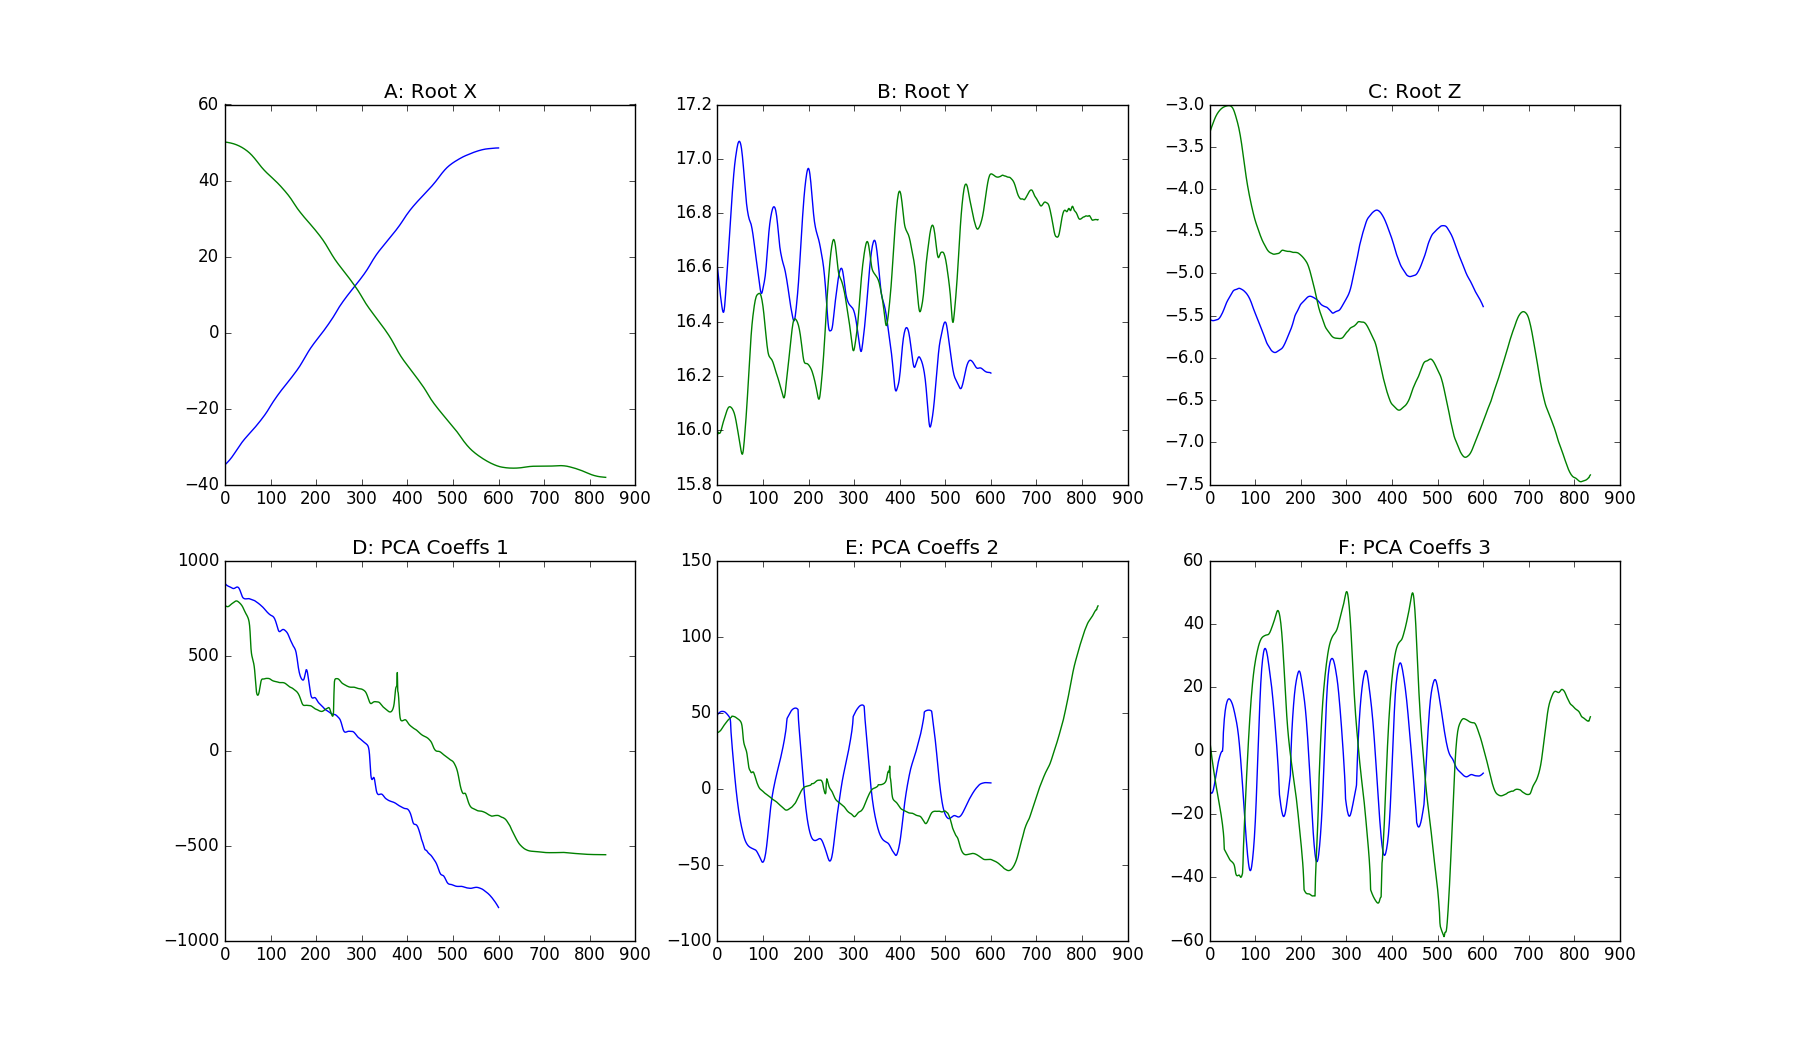
\includegraphics[width=\textwidth]{/home/cshome/j/jcampbell/Desktop/Thesis/Thesis/images/walks.png}
\caption{Motion capture data for a subject as they walk in two different examples. In both cases the subject walked for a short period in one direction and then turned and walked back. The top row shows the position of the root node of the subject while the bottom row shows the data projected according to the PCA basis functions, for each of the first three most significant components. In each of the plots the blue trace is for the first example while the green trace is for the second example. The same subject performed both actions. The two motion examples are 21 and 22 for subject 136 of the CMU Mocap database. \label{walks}}
\end{figure}

\subsection{Motion Capture Data}

In many cases our data will lie in a high-dimensional space. Our input motion capture data, for example, has 59 components, six of which describe the position of the root node over time, while the rest describe the angles of various body joints. There is one joint angle per degree of freedom for each particular joint, however not all joints have the full three degrees of freedom. The joint names and the numbers of degrees of freedom are specified in Fig. {mocap image}.

\subsection{Principle Component Analysis}

Principle component analysis (PCA) is a widely used method for computing a low dimensional representation of data. Given an $n\:\:\text{x}\:\:m$ data matrix $X$, PCA finds a linear transformation to a new set of coordinate axes such that the variance along each of the new axes is maximised. Typically singular value decomposition (SVD) is used to find this transformation. The PCA transform using SVD performs a factorisation of the data matrix according to

\begin{equation}
X = U \Sigma V^{T} 
\end{equation}

\noindent where $U$ and $V$ are the left and right singular vector matrices of size $n\:\:\text{x}\:\:n$ and $m\:\:\text{x}\:\:m$ respectively. The matrix $\Sigma$ is an $n\:\:\text{x}\:\:n$ diagonal matrix containing the $n$ singular values of $X$. The vectors of $V$ are eigenvectors of the covariance matrix $X X^{T}$ and represent the principle components of the transformed data. We transformed data matrix is found by projecting the original data matrix into the space defined by the PCA axes according to

\begin{equation}
Y = V X. 
\label{PCA_compute}
\end{equation}

This method, however, only works efficiently in cases where the dimensionality of each sample is much lower than the number of samples available, i.e. when $n > p$. This is because the covariance matrix $X X^{T}$ becomes very large. 

It is often the case where the dimensionality of our samples is much greater than the number of samples available. We will see in later sections that this is the case for temporal synchronisation of videos. If we represent each frame of a video as a single vector then the dimensionality of each sample is equal to the number of pixels in the image. If our video is only 100 - 200 frames long, then we clearly have $p >> n$. In this situation we turn to an alternative method for estimating the principle components, as defined by reference. 

Since the number of samples is low we can efficiently compute the alternative covariance matrix $X^{T} X$ which is of size $n\:\:\text{x}\:\:n$. We then compute the eigenvalues and eigenvectors of this covariance matrix. The matrix $V$ is formed by stacking the eigenvectors in columns according to the size of the corresponding eigenvalues and can then be used as in Eq. \ref{PCA_compute}.

\subsection{Detecting Frequency}

In this section we will be considering time-series functions of the form

\begin{equation}
f(x) = \sum_i{a_i\sin(b_ix) + c_i\cos(d_ix)}
\end{equation}

\noindent where $a_i$ and $c_i$ are the magnitudes of the two components and $b_i$ and $d_i$ are the frequencies. We will not use this equation explicitly in our algorithm, however it is convenient for demonstrating the attributes of our algorithm.

\begin{figure}[h]
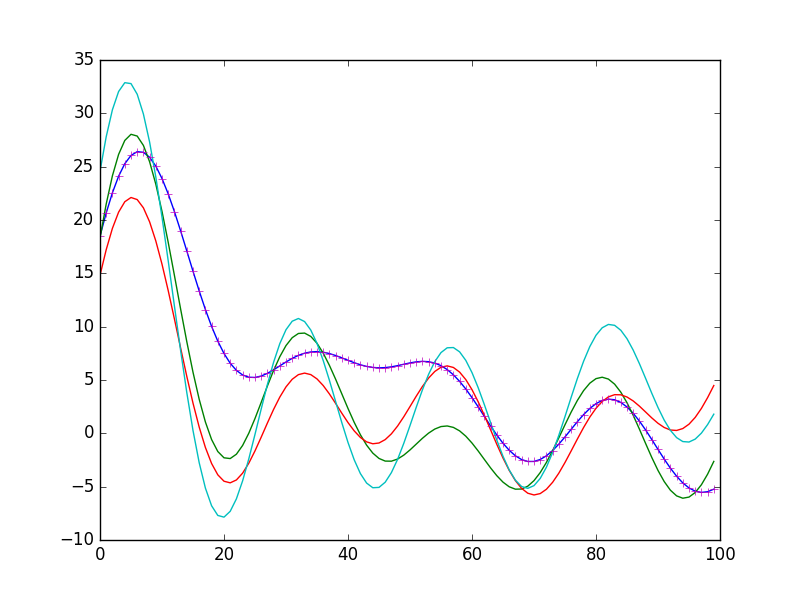
\includegraphics[width=\textwidth]{/home/cshome/j/jcampbell/Desktop/Thesis/Thesis/images/example_waveforms.png}
\caption{Four time-series examples. These may represent joint angles over time, intensity changes of a pixel, or integral curves from an optical flow tracking algorithm, for example. \label{example_waveforms}}
\end{figure}

\section{Temporal Synchronisation}

There are often times when two vides of an activity will not be temporally aligned, for example in film making. In the film industry the term 'shot' is used to denote a short sequence of continuous activity which is not broken by a cut, typically on the order of 1000 frames. It is common for multiple cameras to record each shot, as well as infrared cameras if motion capture technology is being employed. Motion capture systems typically contain their own dedicated hardware temporal synchronisation frameworks, while an additional hardware synchronisation system is employed for the remaining cameras. Hardware synchronisation methods are occasionally used for filming outdoors, however they are often costly and require time to setup for each shoot. Hardware synchronisation methods are therefore inaccessible for amateur cinematographers, and for unplanned, ad hoc recording scenarios. In these situations it is therefore highly likely that the activity recorded from each camera will not be synchronised in time. Furthermore, even if hardware synchronisation has been used, once a shot has been captured it will often be sent to an editorial team, who may perform alterations to the shot which renders the timestamps incorrect. The original and the modified shots will therefore require manual synchronisation to align them again. Manual synchronisation is typically performed by searching for high frequency events such as footfalls, eyeblinks, or when any two items connect. This obviously introduces problems when there is very little scene activity, or when there are no high frequency components. This could occur in tracking shots that produce a sweeping motion, or for shots in which any activity is very smooth, for example a car driving along a street. 

It is vitally important that multiple views of a shot are aligned in time. In live action films it is critical to know when to be able to switch between views, while in films that contain visual effects elements the multiple views are used as input to motion reconstruction pipelines, stereo reconstruction pipelines, and as raw input for artists manually creating creatures and scenes. 

In film making it is often the case that hardware synchronisation methods are used to automatically align video feeds of a scene. 

\section{Activity Clustering}
